\section{Results}\label{sec:results}

\subsection{Task 1: what can text already do?}
A fine-tuned DistilBERT classifier \cite{sanh2019distilbert} reaches macro-F1 \textbf{0.7091}
(micro-F1 0.7503, AUC-PR 0.7302) on MusicCaps tag prediction from captions alone, no audio or
graph involved. Given the 69.1\% lexical exposure measured in Section~\ref{sec:data}, part of
this is a literal shortcut; a caption-sanitization control (target words removed, model
retrained) still recovers 84.3\% of this score, so it is not purely a leakage artifact. Task 2
and 4 use different datasets/metrics, so this is not a numerical baseline they are scored
against -- it is the qualitative anchor that text alone is already strong before any graph is
introduced, the standard the rest of this section's "does the graph add anything" questions
are asked against.

\subsection{Task 2: does topology help audio classification?}\label{sec:results-t2}
\begin{table}[t]
\centering
\caption{Task 2, GTZAN genre classification (150 test tracks). The edge-free encoder uses a
per-node MLP of matched width and depth in place of every GraphSAGE layer, with no edges;
this changes the aggregation operator as well as removing topology, a caveat discussed in
Section~\ref{sec:cross-task}.}
\footnotesize
\begin{tabular}{lcc}
\toprule
Model & Params & Macro-F1 \\
\midrule
CNN (mel-spec., no graph, no text) & -- & \textbf{0.7654} \\
GraphSAGE (deployed, mean-pool) & 13{,}066 & 0.5976 \\
Edge-free, mean-pool$^{\dagger}$ & 6{,}922 & 0.6049 \\
Edge-free, max-pool & 6{,}922 & \textbf{0.6425} \\
Exact 2-hop (fixed aggr., trained head) & 6{,}858 & 0.6630 \\
\bottomrule
\end{tabular}

\vspace{2pt}
{\footnotesize $^{\dagger}$Pooling-matched to the deployed GraphSAGE row above.}
\label{tab:task2-full}
\end{table}
\begin{figure}[t]
\centering
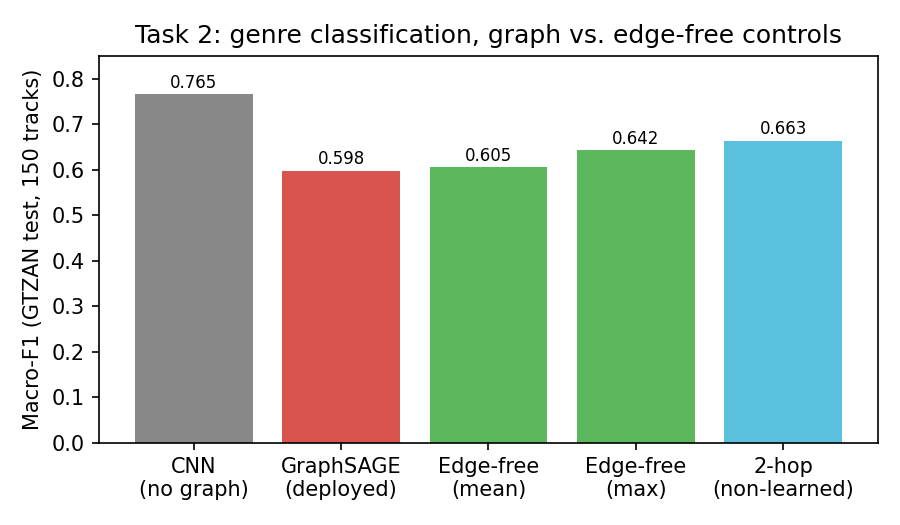
\includegraphics[width=0.8\columnwidth]{figures/fig2_task2_comparison.png}
\caption{Task 2: GTZAN genre classification, graph model vs.\ controls.}
\label{fig:task2}
\end{figure}
The pooling-matched comparison -- both models using mean-pool readout, the fairest single
comparison here -- has the edge-free encoder ahead by \textbf{+0.0072} macro-F1 (0.6049 vs.\
0.5976), using 47\% fewer parameters and no edge information (Figure~\ref{fig:task2}). Its
best result overall, at max-pool, is further ahead (+0.045), but that changes pooling as well
as topology and is not the clean ablation; we report it as the edge-free model's genuine best
result, not the fairest comparison -- neither reading has the graph model ahead. A separate,
repaired, sparser graph construction (mutual $k$-NN, three regimes, three poolings, 8 seeds
each, real vs.\ none/shuffled/random, 27 contrasts \cite{tismir_audit}) likewise found no
training-time contrast favoring the real graph; 18 of the 27 (real-vs-shuffled/random, same
architecture, changing only edge identity) are the topology-only evidence, the remaining 9
(real-vs-none) an edge-free comparison like this paper's own Task 2 control, not
double-counted here. Non-learned exact 2-hop aggregation also beats GraphSAGE, suggesting
part of the gap is GraphSAGE's learned aggregation under-using available signal, not only
weak topology -- a distinction we return to in Section~\ref{sec:discussion}.

\subsection{Task 3: does the graph complement text?}\label{sec:results-t3}
\begin{table}[t]
\centering
\caption{Task 3, MusicCaps fusion (715 test examples, except the edge-free row, which is
validation-only -- see note below).}
\footnotesize
\begin{tabular}{lccc}
\toprule
Mode & Macro-F1 & Micro-F1 & AUC-PR \\
\midrule
bert\_only & \textbf{0.7298} & 0.7647 & 0.7485 \\
gnn\_only (unweighted) & 0.0112 & 0.0290 & 0.0879 \\
gnn\_only (pos-weighted) & 0.1621 & 0.1839 & 0.1196 \\
edge-free gnn, pos-w.\ (max)$^{\dagger}$ & 0.1689 & -- & -- \\
concat & 0.7061 & 0.7478 & 0.7367 \\
cross\_attention & 0.6951 & 0.7398 & 0.7310 \\
\bottomrule
\end{tabular}

\vspace{2pt}
{\footnotesize $^{\dagger}$Validation set, not test -- see Section~\ref{sec:protocol}.}
\label{tab:task3-full}
\end{table}
Text alone (0.7298) outperforms every fusion mode; neither \textit{concat} (0.7061) nor
\textit{cross\_attention} (0.6951) improves on it. The edge-free \textit{gnn\_only} control
was only evaluated on validation, and its pooling-matched comparison does not repeat Task
2's pattern: at mean-pool (matching GraphSAGE's own pooling), the GraphSAGE-equivalent
baseline reaches 0.1640 against the edge-free encoder's 0.1599 -- the graph slightly
\emph{ahead} by +0.0041; only at max-pool does the edge-free encoder lead (0.1689). Both
edge-free readings share the GraphSAGE-equivalent comparator's positive-class weighting,
unlike the Table~\ref{tab:task3-full} rows discussed under Class Weighting
(Section~\ref{sec:protocol}). We report both honestly rather than quote only the max-pool
number: unlike Task 2's, this comparison does not show a clean edge-free advantage once
pooling is fixed, and we do not treat it as this task's primary evidence in either direction
-- that role belongs to the branch-zeroing and complementarity diagnostics below, both on the
real test set and unaffected by this pooling question.

\begin{figure}[t]
\centering
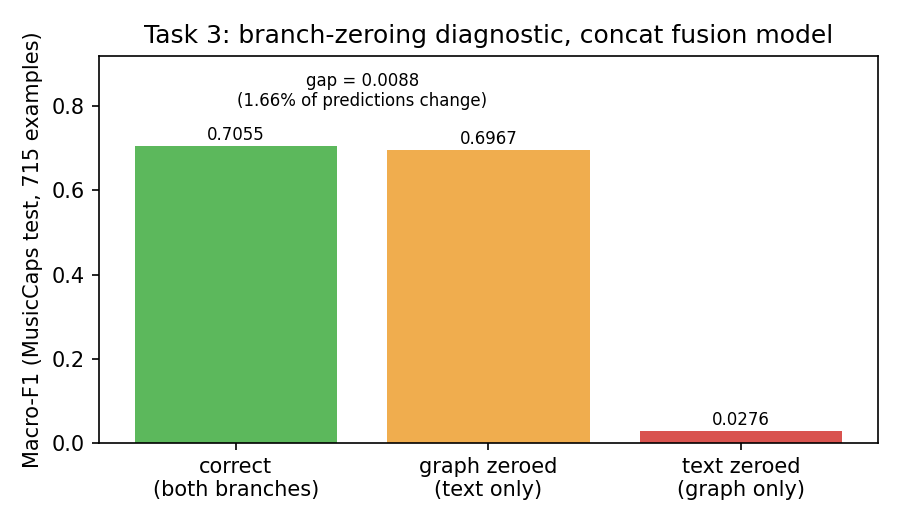
\includegraphics[width=0.8\columnwidth]{figures/fig3_task3_branch_zeroing.png}
\caption{Task 3: branch-zeroing diagnostic on the trained \textit{concat} fusion model.}
\label{fig:task3}
\end{figure}

\textbf{Branch-zeroing} (Figure~\ref{fig:task3}): replacing the
graph embedding with zeros inside the trained \textit{concat} model changes only
\textbf{1.66\%} of individual (example, tag) predictions and costs \textbf{0.0088} macro-F1
(0.7055 $\to$ 0.6967; 0.7055 is this diagnostic run's own re-measurement of \textit{concat},
negligibly different from Table~II's 0.7061); zeroing the text branch instead costs 0.6779
macro-F1, confirming text is overwhelmingly informative. This 0.0088 comes from the primary
evidence base (Section~\ref{sec:data}). The accompanying repository's own
\texttt{src/task3\_branch\_zeroing.py} instead reports 0.1205 (archived at
\texttt{results/task3\_branch\_zeroing.json}), against a \textit{concat} checkpoint that
repository's own training produced on its 673-example, 30-tag split -- a trained artifact not
itself shipped there, so a fresh clone cannot rerun this exactly without retraining, and
retraining is not guaranteed to reproduce 0.1205 given the non-determinism
Section~\ref{sec:discussion} discloses. Despite sharing this script's name, it runs a
different implementation, different data, and a differently trained checkpoint, part of a
disclosed follow-up that did not confirm this reading (Section~\ref{sec:discussion}) -- the
two numbers are not interchangeable, named explicitly rather than let the shared filename
imply otherwise.

\textbf{Complementarity}: cross-tabulating \textit{bert\_only} against \textit{gnn\_only}
predictions -- two separately-trained, single-branch models, not the fusion model
(35{,}750 cells, 715 examples $\times$ 50 tags) -- using the standard, unweighted
\textit{gnn\_only} checkpoint (macro-F1 0.0112) finds the graph model correct on 508 of
1{,}047 cells where text is wrong (\textbf{48.5\%}, an apparent "rescue rate"). Taken at face
value this looks like real, modest complementary signal. It is not: this checkpoint's
precision/recall (Table~\ref{tab:task3-full}) are exactly 0.0 for 45 of 50 tags -- it
predicts positive for only 5 -- so most "correct" cells are true negatives from never
predicting positive, not audio-based detection. Splitting the 508 by label polarity (the same
check applied to the accompanying repository's own numbers, Section~\ref{sec:discussion})
confirms this: only \textbf{3 of 508} (0.6\%) are genuine true positives where text was a
false negative; the remaining \textbf{505 of 508} (99.4\%) are the graph model defaulting to
"absent" while text wrongly said "present." An always-predict-absent classifier would, by
construction, rescue the same 509-of-1{,}047 (48.6\%) -- essentially the observed 48.5\%, so
this headline number does not distinguish the checkpoint from a trivial one and is not read
as complementary signal; it is also outnumbered by the reverse 1{,}735 cells where text is
right and the graph wrong. This cross-tabulation is correlational, comparing two
independently trained models. Branch-zeroing above is a narrower causal intervention: it
manipulates the trained fusion model's input at inference and measures the output effect,
distinct from a training-time test of a graph-absent-from-the-start model (zero may be an
input the model never saw, so this measures reliance as currently trained, not causal
contribution under retraining). With that scope, it found removing the graph costs only
0.0088 macro-F1 -- small, but genuine, a more direct kind of evidence than complementarity's
correlational count. One further, tentative point: richer pretrained node features (frozen
CNN embeddings trained for GTZAN genre, replacing chroma+MFCC) give a modest single-seed,
validation-only gain (0.1640 $\to$ 0.1846, +0.0206) -- a hint that node-feature weakness is
part of the story, but one run, a mismatched embedding source, no test-set or multi-seed
confirmation.

\subsection{Task 4: does any graph benefit survive under retrieval?}\label{sec:results-t4}
\begin{table}[t]
\centering
\caption{Task 4, MusicCaps retrieval (673 test examples), mean $\pm$ population standard
deviation (\texttt{ddof=0}) over 3 seeds.}
\begin{tabular}{lcc}
\toprule
Metric & Real graph & Edge-free \\
\midrule
Audio$\to$Text R@1  & 0.0124 $\pm$ 0.0019 & 0.0124 $\pm$ 0.0046 \\
Audio$\to$Text R@5  & 0.0570 $\pm$ 0.0062 & 0.0589 $\pm$ 0.0046 \\
Audio$\to$Text R@10 & 0.1025 $\pm$ 0.0053 & 0.1000 $\pm$ 0.0091 \\
Text$\to$Audio R@1  & 0.0099 $\pm$ 0.0031 & 0.0104 $\pm$ 0.0032 \\
Text$\to$Audio R@5  & 0.0515 $\pm$ 0.0037 & 0.0570 $\pm$ 0.0101 \\
Text$\to$Audio R@10 & 0.1030 $\pm$ 0.0125 & 0.1010 $\pm$ 0.0063 \\
\bottomrule
\end{tabular}
\label{tab:task4-full}
\end{table}
\begin{figure}[t]
\centering
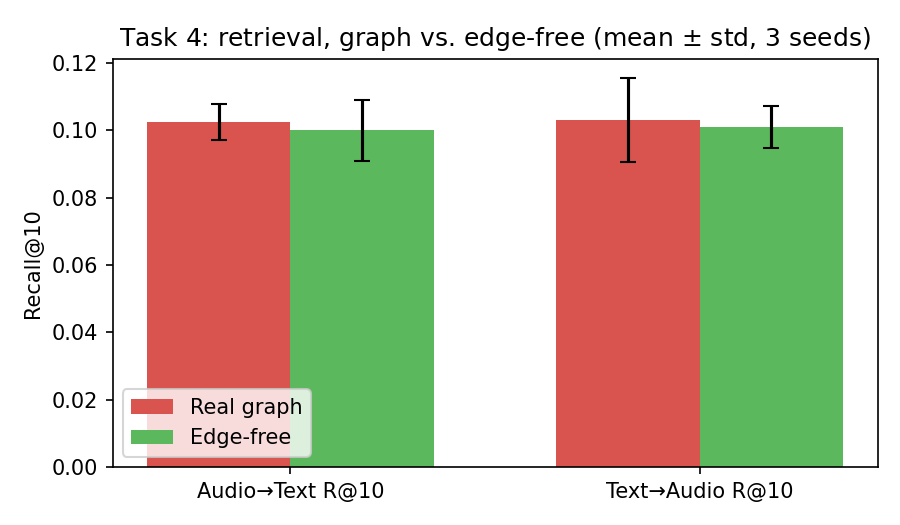
\includegraphics[width=0.8\columnwidth]{figures/fig4_task4_retrieval.png}
\caption{Task 4: retrieval Recall@10, graph vs.\ edge-free encoder.}
\label{fig:task4}
\end{figure}
Across three training seeds, the absolute difference between the real-graph and edge-free
encoders' means ranges from 0.00000 to 0.00545 across the six reported metrics
(Figure~\ref{fig:task4}) -- smaller, on every metric, than at least one condition's own
population standard deviation (ddof=0), though not always both, so we avoid the imprecise
"within one SD" description. With only three runs and no significance/equivalence test, the
defensible statement is no consistent advantage for either encoder in either direction, not
proof of equivalence. This is more informative than an earlier single-seed check, which
showed edge-free ahead on audio$\to$text R@10 by 0.028 and graph-based ahead on
text$\to$audio R@10 by 0.015 -- neither gap recurs in the three-seed rerun (per-seed gaps
range only $-0.013$ to $+0.021$ and $-0.006$ to $+0.010$ respectively, narrower in both
directions), though three seeds is too small a basis to call this an established difference
in variability, only a description of what these runs showed.
Zero-shot tag prediction (embedding tag names as text, no supervised classifier;
Section~\ref{sec:protocol}) reaches macro-F1 0.146 on the single seed-42 real-graph
checkpoint -- not the three seeds behind Table~\ref{tab:task4-full}, and without a
random-encoder control to confirm this is above chance, so we report it without the stronger
"confirms semantic content" claim it might otherwise support. It is, as expected, far below
Task 1's supervised classifier, for a system that never sees tag or genre labels during
training (it sees which caption pairs with which clip, a form of supervision, just not a
tag/genre label). In a separate, single-seed check on the real-graph encoder, quadrupling the
contrastive batch size (32$\to$128) changed R@10 by at most 0.006 in either direction --
suggestive against batch size being the bottleneck, though not repeated for the edge-free
encoder or across seeds, so a secondary observation, not a controlled result on the same
footing as the comparison above.

\textbf{Qualitative failure review.} A possible objection to exact-pair retrieval evaluation
is that a "wrong" top-1 result might still be semantically reasonable, just not the official
paired clip -- a false negative of the protocol, not a model error. We inspected 20
successes (true clip in the top 3) and 20 failures (below 10th) manually, comparing each
failure's query caption against its top-1 match's caption. The failures are not close
misses: median rank 166 of 673, ranging 28-352 across the 20 (individual ranks archived
alongside this evaluation). Reading the caption pairs, the large majority describe clearly
different instrumentation, genre, or mood (e.g.\ a piano-and-propeller query's top-1 match
was a Russian lullaby with vocals). A small number share a coarse category (both
instrumental, or reverb-heavy) without matching specific content. We do not find evidence
that exact-pair evaluation hides a large population of semantically-correct-but-unpaired
matches; most failures are genuine retrieval errors. Real limits: the 40 examples are the
first qualifying test cases in dataset order, not a random sample, judged by one author
without a blinded rater or predefined rubric -- a manual sanity check, not a formal
annotation study.
